% !TeX spellcheck = ru_RU
\documentclass[a4paper,12pt]{extarticle}
\usepackage[utf8x]{inputenc}
\usepackage[T1,T2A]{fontenc}
\usepackage[russian]{babel}
\usepackage{hyperref}
\usepackage{indentfirst}
\usepackage{listings}
\usepackage{color}
\usepackage{here}
\usepackage{array}
\usepackage{multirow}
\usepackage{graphicx}

\usepackage{caption}
\renewcommand{\lstlistingname}{Программа} % заголовок листингов кода

\bibliographystyle{ugost2008ls}

\usepackage{listings}
\lstset{ %
extendedchars=\true,
keepspaces=true,
language=C,						% choose the language of the code
basicstyle=\footnotesize,		% the size of the fonts that are used for the code
numbers=left,					% where to put the line-numbers
numberstyle=\footnotesize,		% the size of the fonts that are used for the line-numbers
stepnumber=1,					% the step between two line-numbers. If it is 1 each line will be numbered
numbersep=5pt,					% how far the line-numbers are from the code
backgroundcolor=\color{white},	% choose the background color. You must add \usepackage{color}
showspaces=false				% show spaces adding particular underscores
showstringspaces=false,			% underline spaces within strings
showtabs=false,					% show tabs within strings adding particular underscores
frame=single,           		% adds a frame around the code
tabsize=2,						% sets default tabsize to 2 spaces
captionpos=t,					% sets the caption-position to top
breaklines=true,				% sets automatic line breaking
breakatwhitespace=false,		% sets if automatic breaks should only happen at whitespace
escapeinside={\%*}{*)},			% if you want to add a comment within your code
postbreak=\raisebox{0ex}[0ex][0ex]{\ensuremath{\color{red}\hookrightarrow\space}},
texcl=true,
inputpath=listings,                     % директория с листингами
}

\usepackage[left=2cm,right=2cm,
top=2cm,bottom=2cm,bindingoffset=0cm]{geometry}

%% Нумерация картинок по секциям
\usepackage{chngcntr}
\counterwithin{figure}{section}
\counterwithin{table}{section}

%%Точки нумерации заголовков
\usepackage{titlesec}
\titlelabel{\thetitle.\quad}
\usepackage[dotinlabels]{titletoc}

%% Оформления подписи рисунка
\addto\captionsrussian{\renewcommand{\figurename}{Рисунок}}
\captionsetup[figure]{labelsep = period}

%% Подпись таблицы
\DeclareCaptionFormat{hfillstart}{\hfill#1#2#3\par}
\captionsetup[table]{format=hfillstart,labelsep=newline,justification=centering,skip=-10pt,textfont=bf}

%% Путь к каталогу с рисунками
\graphicspath{{fig/}}

\usepackage{minted}

\begin{document}	% начало документа

% Титульная страница
\begin{titlepage}	% начало титульной страницы

	\begin{center}		% выравнивание по центру

		\large Санкт-Петербургский политехнический университет Петра Великого\\
		\large Институт компьютерных наук и технологий \\
		\large Кафедра компьютерных систем и программных технологий\\[6cm]
		% название института, затем отступ 6см
		
		\huge Телекоммуникационные технологии\\[0.5cm] % название работы, затем отступ 0,5см
		\large Отчет по лабораторной работе №7\\[0.1cm]
		\large Помехоустойчивое кодирование\\[5cm]

	\end{center}


	\begin{flushright} % выравнивание по правому краю
		\begin{minipage}{0.25\textwidth} % врезка в половину ширины текста
			\begin{flushleft} % выровнять её содержимое по левому краю

				\large\textbf{Работу выполнил:}\\
				\large Графов Д.И.\\
				\large {Группа:} 33531/2\\
				
				\large \textbf{Преподаватель:}\\
				\large Богач Н.В.

			\end{flushleft}
		\end{minipage}
	\end{flushright}
	
	\vfill % заполнить всё доступное ниже пространство

	\begin{center}
	\large Санкт-Петербург\\
	\large \the\year % вывести дату
	\end{center} % закончить выравнивание по центру

\thispagestyle{empty} % не нумеровать страницу
\end{titlepage} % конец титульной страницы

\vfill % заполнить всё доступное ниже пространство


% Содержание
% Содержание
\renewcommand\contentsname{\centerline{Содержание}}
\tableofcontents
\newpage




\section{Цель работы}
Познакомиться со средствами генерации и визуализации простых сигналов.

\section{Программа работы}
С помощью языка программирования Python и его библиотек
промоделировать синусоидальный и прямоугольный сигналы с различными параметрами. Получить их спектры. Вывести на график.

\section{Теоретическая информация}
Среди множества библиотек Python выделим основные, используемые для математических расчётов и визуализации.
\begin{itemize}
	\item \textbf{NumPy} -- это open-source модуль для Python, который предоставляет общие математические и числовые операции в виде пре-скомпилированных, быстрых функций. Они объединяются в высокоуровневые пакеты. Они обеспечивают функционал, который можно сравнить с функционалом MatLab. NumPy (Numeric Python) предоставляет базовые методы для манипуляции с большими массивами и матрицами. SciPy (Scientific Python) расширяет функционал numpy огромной коллекцией полезных алгоритмов, таких как минимизация, преобразование Фурье, регрессия, и другие прикладные математические техники.
	
	\item \textbf{Matplotlib} — библиотека на языке программирования Python для визуализации данных двумерной (2D) графикой (3D графика также поддерживается). Получаемые изображения могут быть использованы в качестве иллюстраций в публикация.
	
	Генерируемые в различных форматах изображения могут быть использованы в интерактивной графике, в научных публикациях, графическом интерфейсе пользователя, веб-приложениях, где требуется построение диаграмм (англ. plotting). В документации автор признаётся, что Matplotlib начинался с подражания графическим командам MATLAB, но является независимым от него проектом.
	
	Библиотека Matplotlib построена на принципах ООП, но имеет процедурный интерфейс pylab, который предоставляет аналоги команд MATLAB.
	
	\item \textit{Сигнал} - это физическое явление, служащее для передачи информации, которое может иметь различную природу. Должен также иметь различимые состояния (минимум 2), чтобы передавать информацию (например, наличие сигнала и его отсутствие).
	
	\item \textit{Спектр сигнала} - это результат разложения сигнала на более простые в базисе ортогональных функций. В качестве разложения обычно используются преобразование Фурье и другие.
	
	\begin{center}
		В радиотехнике в качестве базисных функций используют синусоидальные функции. Это объясняется рядом причин:
	\end{center}
	\item функции $ cos(\omega t) $, $ sin(\omega t)$ являются простыми и определены при всех значениях \textit{t}, являются ортогональными и составляют полный набор при кратном уменьшении периода;
	\item гармоническое колебание является единственной функцией времени, сохраняющей свою форму при прохождении колебания через линейную систему с постоянными параметрами, могут только изменяться амплитуда и фаза;
	\item для гармонических функций имеется математический аппарат комплексного анализа;
	\item гармоническое колебание легко реализуемо на практике. 
	
	\item Спектр сигнала $s(t)$ можно записать через преобразование Фурье (можно без коэффициента $ 1/{\sqrt {2\pi }}$) в виде:
	
	$ S(\omega )=\int_{-\infty }^{+\infty }s(t)e^{-i\omega t}dt $, где $\omega $ - угловая частота равная $ 2\pi f $.
	
	Спектр сигнала является комплексной величиной и представляется в виде: \\
	$ S(\omega )=A(\omega )e^{-i\phi (\omega )}$, где $A(\omega )$ - амплитудно-частотная характеристика сигнала, $\phi (\omega ) $ - фазо-частотная характеристика сигнала.
	\end {itemize}

\section{Ход выполнения работы}
На языке python мной была написана программа, генерирующая синусоидальный и прямоугольный сигналы, а также отобразить их спектры.

\subsection{Листинг 1. main.py}
\inputminted[
frame=lines,
framesep=2mm,
baselinestretch=1.2,
fontsize=\footnotesize,
linenos
]{python}{../src/main.py}

\subsection{Результат работы}

\begin{figure}[H]
	\begin{center}
		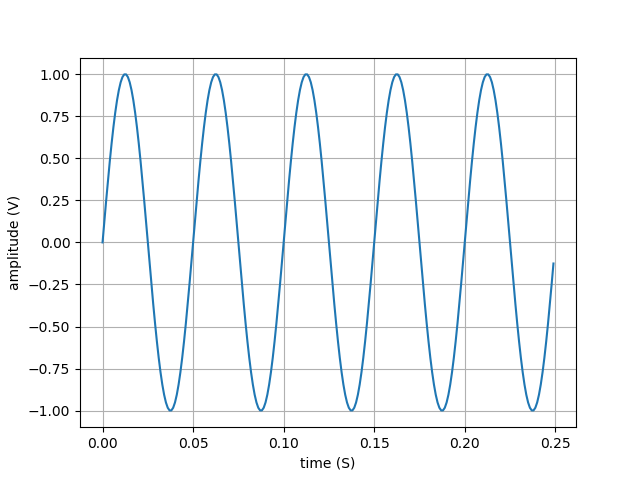
\includegraphics[scale=0.7]{../out/sine_time.png}
		\caption{Синусоидальный сигнал} 
		\label{pic:sine_time} % название для ссылок внутри кода
	\end{center}
\end{figure}

\begin{figure}[H]
	\begin{center}
		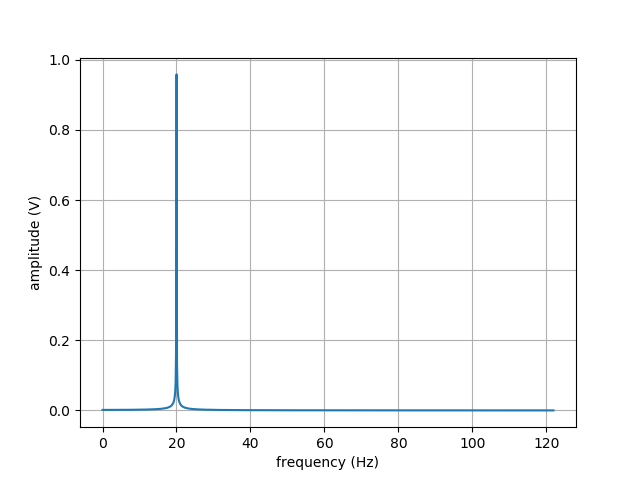
\includegraphics[scale=0.7]{../out/sine_freq.png}
		\caption{Спектр синусоидального сигнала} 
		\label{pic:sine_freq} % название для ссылок внутри кода
	\end{center}
\end{figure}

\begin{figure}[H]
	\begin{center}
		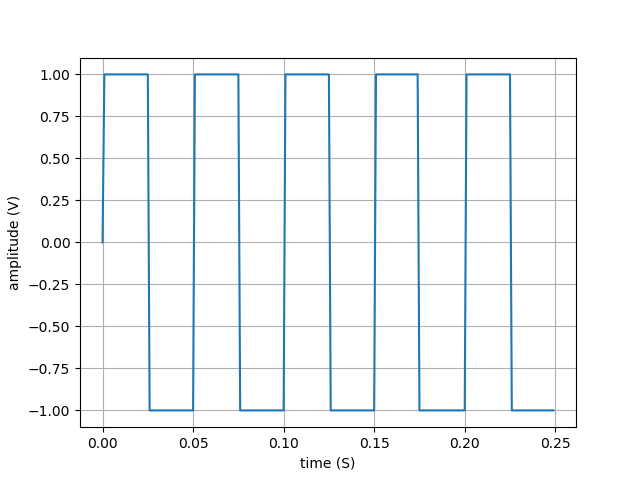
\includegraphics[scale=0.7]{../out/square_time.png}
		\caption{Прямоугольный сигнал} 
		\label{pic:square_time} % название для ссылок внутри кода
	\end{center}
\end{figure}

\begin{figure}[H]
	\begin{center}
		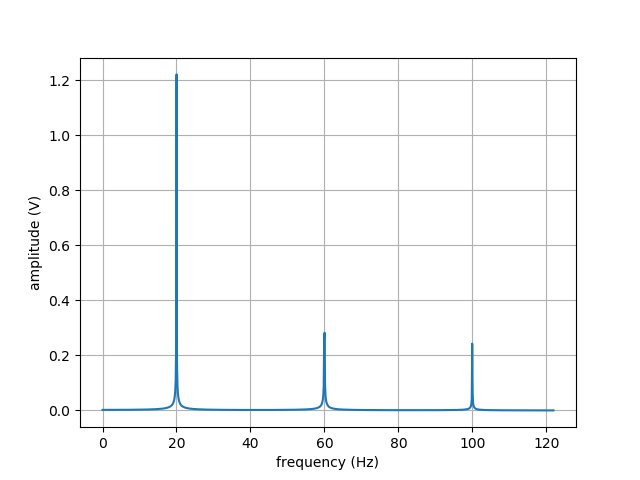
\includegraphics[scale=0.7]{../out/square_freq.png}
		\caption{Спектр прямоугольного сигнала} 
		\label{pic:square_freq} % название для ссылок внутри кода
	\end{center}
\end{figure}

\newpage
\section{Выводы}
В данной лабораторной работе по курсу "Телекоммуникационные технологии" мной были промоделированы синусоидальный и прямоугольный сигналы, а также получены их спектры.

Сигналы бывают периодические и непериодические. Для периодических сигналов выполняется общее условие $ s(t) = s(t + kT)$, где $k = 1, 2, 3, ...$ - любое целое число, $Т$ - период, являющийся конечным отрезком независимой переменной.

В данной лабораторной работе мной выяснено, что периодический сигнал имеет дискретный спектр. Если же сигнал не периодический, то спектр в этом случае будет непрерывным.
\end{document}
